\chapter{De blockchain technologie}\label{chap:q1}
In dit hoofdstuk wordt er een korte uitleg gegeven over een aantal basis technische termen in cryptografie, blockchain-technologie en gerelateerde concepten zoals smart contracts. Dit zodat we weten waar we het over hebben wanneer we het proof of concept behandelen.

\section{Het algemene concept achter de blockchain}
Blockchain technlogie is bekend geworden door de introductie van de digitale valuta bitcoin. De bitcoin werd geintroduceerd door Satoshi Nakamoto in 2008 door een white paper genaamed Bitcoin: A Peer-To-Peer Electronic Cash System \cite{bitcoinPaper}. Hierin legt hij uit hoe in een peer-to-peer omgeving geld overgemaakt kan worden om online betalingen rechtstreeks van de ene partij naar de andere overgemaakt kunnen worden, zonder een financiële instelling. De blockchain is de technologie achter de Bitcoin die het mogelijk maakt.\par

In dit onderzoek gebruiken we de beschrijving het ICTU \footnote{https://www.ictu.nl/}, die de blockchain beschrijft als: een specifieke databasetechnologie die leidt tot een gedistribueerd autonoom grootboeksysteem \cite{kaptijn}. De integriteit van dit gedistribueerd autonoom grootboeksysteem wordt gewaarborgd doordat iedere partij zeggenschap heeft bij de validatie van een transactie. Dit versnelt het proces doordat beheerders en tussenpersonen worden uitgeschakeld. Meningsverschillen worden opgelost door een consensus van een meerderheid van de deelnemers.\par

Databasetransacties worden gegroepeerd in data blokken die vervolgens achter elkaar in een reeks blokken worden opgeslagen, vandaar de naam blockchain. De koppeling tussen blokken en hun inhoud wordt beschermd door cryptografie en kan niet worden vervalst. Daarom kan informatie die eenmaal in een blockchain is ingevoerd niet worden gewist; In essentie bevat een blockchain een accuraat, tijd gestempeld en verifieerbaar archief van elke transactie die ooit is gemaakt. Figuur \ref{fig:blockchain?} geeft het algemene idee weer van hoe deze technologie werkt met als bekende use case de bitcoin.
\begin{figure}
    \begin{center}
        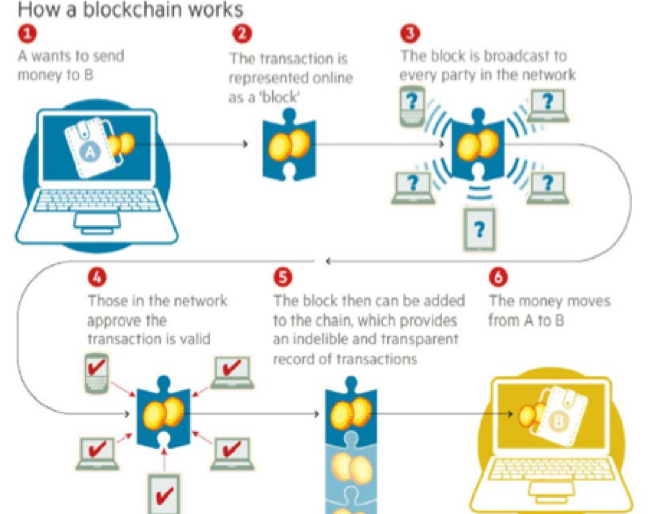
\includegraphics[scale=0.80]{images/blockchain?}
        \caption{Illustreert hoe de blockchain werkt \cite{howBlockchainWorks}}
        \label{fig:blockchain?}
    \end{center}
\end{figure}
\newpage

De blockchain technologie lost verschillende problemen op die voorkomen bij het gebruik van traditionele gecentraliseerde database technologieën die in handen zijn van één instantie. Dit soort technologieën vereisen vertrouwen dat de beheerder zorgvuldig omgaat met de toegang of bewerkingen van de data. Verder dat de database toegankelijk is voor de belanghebbenden en dat de instantie er de volgende dag nog is. Deze problemen komen niet voor in een gedecentraliseerde blockchain database. Dit komt omdat een nieuwe dienst, software bedrijf of markten op de blockchain de volgende zes design principes \cite{blockRev} hanteren:
\begin{enumerate}
	\item Netwerk integriteit\\
	Het systeem bewaakt de data integriteit doordat ieder lid in het netwerk alle transacties kan nalopen en kan controleren. Inplaats dat er maar een lid is dit proces uitvoert. Gebruikers op het netwerk kunnen rechtstreeks waarde met elkaar uitwisselen door dit te registeren op een blok. Elk blok heeft een verwijzing naar een voorgaand blok verwijzen, waardoor niemand een transactie kan verbergen of kan vervalsen. Dit omdat er meer andere gebruikers zijn met de juiste realiteit.
	\item Gedistribueerd\\
	Het systeem is volledig Gedistribueerd. Dit houd in dat er geen één punt is van controle. Er is niet een gebruiker of organisatie die het systeem uit kan zetten.
	\item Security\\
	In Satoshi’s white paper \cite{bitcoinPaper}, geeft hij aan dat iedere deelnemen van het netwerk vereist zijn om een public key infrastructure (PKI) te gebruiken om het platform veilig te houden. De PKI is een geavanceerde vorm van asymmetrische cryptografie, waar de gebruiker beide een publiek en privé sleutel ontvangt om zichzelf binnen het netwerk te identificeren en berichten kan versleutelen en onsleutelen.
	\item Eigendomsrechten\\
	Eigendomsrechten zijn transparant en afdwingbaar voor iedere gebruiker. Hierdoor dient een blockchain als een publiek register. Door een tool die Proof of Existence (PoE) heet. Deze tool creert en registeert de cryptografische overzichten van akten, licenties en andere rechten van gebruikers. Dit word gedaan door een hash te berekenen van de public key van een gebruiker.
	\item Privacy\\
	Gebruikers beheren hun eigen data. Er is geen centrale partij die dit doet. Op een blockchain netwerk kunnen gebruikers er zelf voor kiezen wat zij vrij geven aan persoonlijke informatie. Dit kan worden gedaan door persoonlijke gegeven mee te geven in hun public key of in een externe centrale database. Het gehele identificatie en verificatie laag die ervoor weggeeft wie wat naar elkaar stuurt is los van het de transactie laag. Hierdoor kunnen gebruikers op de blockchain anoniem zijn.	
	\item Valuta als motivatie\\
	Het systeem motiveert deelnemers van het netwerk door ze valuta te geven voor bepaalde acties op het netwerk. In het geval van de bitcoin, krijgen miners bitcoin geld voor het eerst volgende blok te koppelen aan het vorige blok aan data. Dit wordt gedaan door een cryptografische puzzel op te lossen die geleidelijk lastiger word.
\end{enumerate}
\newpage

\section{Type Blockchain}
Om een geïnformeerd besluit te maken welk type blockchain juist is voor het proof of concept worden de verschillende type blockchain in dit paragraaf behandeld. Dit word gedaan vanaf een hoog technisch niveau. In essentie zijn er drie types blockchain: privé, consortium en openbaar. Deze types kunnen daarna weer onderverdeeld worden in twee categorieën: open bevat openbaar en gesloten bevat privé en consortium. \par

De categorie gesloten, waarin de types privé en consortium zitten zijn bedoelt voor een gelimiteerde omgeving zoals een bedrijf of groepen bedrijven en organisaties. Terwijl een openbare blockchain een open is tot iedereen er geen permissies zijn die mensen of systemen erbuiten houden.\par

Per type blockchain word er ook gelijk gekeken naar de grote projecten die relevant zijn. Zodat in een vervolg hoofdstuk hierover een vergelijking kan worden uitgevoerd.

\subsection{Privé Blockchain}
Voor een volledige private blockchain, moeten de schrijf rechten op een centrale plek staan die beheert word vaak door een organisatie. De lees rechten kunnen beide publiekelijk of ook net zo beperkt zijn als de schrijf rechten. Applicaties die gebruik maken van een privé Blockchain zijn interne apps die alleen gebruikt worden binnen een bedrijf of organisatie. Want in andere gevallen word publieke lees rechten en controleerbaarheid vereist \cite{privateBlockChains}. Voorbeelden van privé Blockchains zijn MultiChain en Hyperledger:

\textbf{MultiChain} - MultiChain is een platform voor het ontwikkelen en publiceren van privé blockchains. Het lost een aantal schaalbaarheid problemen \cite{oreillyScalability} van de blockchain op met een geinteregeerde gebruiker permissie systeem. Verder bied het bedrijven de mogelijkheid om zonder software ontwikkelaars een blockchain op te richten \cite{mutlichain}.

\textbf{Hyperledger} - Hyperledger is een open source project die ontwikkeld word met het doel om een geavanceerd bedrijfstakoverkoepelende blockchain implementatie te ontwikkelen. Het word gehost door de Linux Foundation \cite{linuxFoundation} en wordt gezamelijk ontwikkeld door grote organisatie in financiën, banken, IoT, productie en technologie \cite{hyperledger}. 

\subsection{Consortium Blockchain}
Consortium blockchain is gedeeltelijk Privé. Het Overeenstemmingproces ookwel consensusproces over de integriteit van de data op de blockcahin wordt door een aantal voorafgeselecteerde nodes (gebruikers) uitgevoerd. Deze nodes zijn bijvoorbeeld 10 grote financiële instellingen die bij de aanmaak van een nieuwe block aan de blockchain zeggenschap hebben. Andere deelnemers van de blockchain hebben nogsteeds het recht om de besluiten van de 10 nodes te controlleren, maar ze hebben verder geen stem in het feit of de volgende block valide is.\par

Het voordeel van de consortium variant is deze efficiënter zijn en toch voldoende transactie transparantie geven. Ook is het niet een bedrijf die alleen oordeelt over de data. Voorbeelden van dit type zijn Ethereum en R3:

\textbf{Ethereum} - Het Ethereum project beschrijft zich als een gedecentraliseerd platform voor applicaties die precies gedraait worden zoals ze geprogrammeerd worden zonder enige kans van fraude, censuur of veranderingen van derden \footnote{https://www.ethereum.org/}. Applicaties, smart contracts, worden geprogrammeerd in de Solidity taal die voor het Ethereum project is ontwikkeld. Het word open-source ontwikkeld en er is een bondgenootschap, de Enterprise Ethereum Alliance \footnote{https://entethalliance.org/} dat bestaat uit 315 furtune 500 bedrijven en organisaties, die gezamelijk werken aan het het enige platform die smart contracts ondersteund op de blockchain.\cite{ethWood}\par

Het project kan gezien worden als verder uitgewerkte versie van Bitcoin die meer functionaliteiten toevoegt. Zo bestaat de status van Ethereum netwerk net zoals de Bitcoin uit meerdere objecten die 'accounts' worden genoemd, waarbij elke account een adres van 20 bytes en statusovergangen heeft. De staat van deze objecten worden opgeslagen in de blockchain waaruit gelijk afgeleiden kan worden waar valuta naartoe gaat.\cite{whitePaperEthereum}

\textbf{R3} - Dit is een gedistribueerd database-technologiebedrijf in New York. Het is verbonden met veel van 's werelds grootste financiële instellingen, met als missie om de voordelen van de blockchain te realiseren \cite{R3}.

\subsection{Openbare Blockchain}
Dit type blockchain is zoals de naam al aangeeft publiek beschikbaar tot iedereen in de wereld. Dit houd in tegenstelling tot Consortium ook het consensusproces in. Iedere gebruiker op het netwerk heeft zeggenschap op de geldigheid van nieuwe data en kan nieuwe data schrijven. \par

Een volledig publieke blockchain is een open-source systeem door het gebruik van zogeheete cryptoeconomics gebruikers op economisch doeleinde motiveert om samen te werken. Hierdoor kunnen ontwikkelaars die gebruik maken van zo'n blockchain belangen zoals beschikbaarheid waarborgen. Bijvoorbeeld zorgt een hogere tarief in een transactie resulteren in snellere transacties of convergentie over de nieuwe blokken die toegevoegd worden aan de blockchain. Een voorbeeld van hiervan is het bekende Bitcoin project.

\textbf{Bitcoin}. Bitcoin is het bekenste voorbeeld van een blockchain project. Bitcoin staat vooral bekend als digitale valuta en online betalingssysteem die door gebruik van cryptografie om valuta-eenheden te geneert en reguleert. Verder gebruikt het cryptografie om de overdracht van fondsen te verifiëren zonder een centrale bank. \par

\newpage